%% ****** Start of file apstemplate.tex ****** %
%%
%%
%%   This file is part of the APS files in the REVTeX 4.2 distribution.%%
%%   Copyright (c) 2024 The American Physical Society.
%%
%%   See the REVTeX 4 README file for restrictions and more information.
%%
%
% This is a template for producing manuscripts for use with REVTEX 4.2
% Copy this file to another name and then work on that file.
% That way, you always have this original template file to use.
%
% Group addresses by affiliation; use superscriptaddress for long
% author lists, or if there are many overlapping affiliations.
%  N.B. The groupedaddress option will reorder the author list based
%  on the order in which affiliations appear. Please be sure to check the author 
%  order. You can also use the unsortedaddress(?) option instead to prevent that
%  behavior.
% For Phys. Rev. appearance, change preprint to twocolumn.
% Choose physrev, prl, or rmp for journal
%  N.B. physrev is appropriate for all APS journals except prl and rmp
%  Add 'draft' option to mark overfull boxes with black boxes
%  Add 'showkeys' option to make keywords appear
\documentclass[aps,physrev,preprint,groupedaddress,linenumbers]{revtex4-2}
%\documentclass[aps,physrev,preprint,superscriptaddress]{revtex4-2}
%\documentclass[aps,prl,preprint,superscriptaddress]{revtex4-2}
%\documentclass[aps,prl,reprint,groupedaddress]{revtex4-2}
%\documentclass[aps,rmp,preprint,superscriptaddress]{revtex4-2}
%\documentclass[aps,rmp,reprint,groupedaddress]{revtex4-2}

% You should use BibTeX and apsrev.bst for references
% Choosing a journal automatically selects the correct APS
% BibTeX style file (bst file), so only uncomment the line
% below if necessary.
\bibliographystyle{apsrev4-2}

% Packages
\usepackage{graphicx}
\usepackage{amsmath}
\usepackage{amssymb}
\usepackage[english]{babel}
\usepackage{hyperref}
\usepackage{xcolor}
\begin{document}

% Use the \preprint command to place your local institutional report
% number in the upper righthand corner of the title page in preprint mode.
% Multiple \preprint commands are allowed.
% Use the 'preprintnumbers' class option to override journal defaults
% to display numbers if necessary
%\preprint{}

%Title of paper
\title{\textbf{Scaling behaviors in simulated collagen fibrils}}

\author{Robert Bertoldo Tavares}
\affiliation{Departamento de Física, Universidade Federal do Ceará, Fortaleza, Ceará, Brasil}

\author{Michael Ferreira de Souza}
\affiliation{Departamento de Estatística e Matemática Aplicada, Universidade Federal do Ceará, Fortaleza, Ceará, Brasil}

\author{B\'ela Suki}
\affiliation{Department of Biomedical Engineering, Boston University, Boston, MA, USA}

\author{Ascânio Dias Araújo}
 \email{ascanio@fisica.ufc.br}
\affiliation{Departamento de Física, Universidade Federal do Ceará, Fortaleza, Ceará, Brasil}
\affiliation{Departamento de Estatística e Matemática Aplicada, Universidade Federal do Ceará, Fortaleza, Ceará, Brasil}

%Collaboration name if desired (requires use of superscriptaddress
%option in \documentclass). \noaffiliation is required (may also be
%used with the \author command).
%\collaboration can be followed by \email, \homepage, \thanks as well.
%\collaboration{}
%\noaffiliation

\date{\today}

\begin{abstract}
Collagen fibrils are hierarchical protein assemblies that provide tensile strength and structural support to mammalian tissues. Understanding the relationship between assembly kinetics, structural organization, and mechanical properties is fundamental to soft matter physics and biomaterials science. Here, we investigate the formation of collagen fibrils using a diffusion-limited aggregation (DLA) model incorporating a surface diffusion parameter $T_s$, which minimize exposed surface area. Our findings indicate that $T_{s}$  governs the morphological transition from fractal aggregates to compact structures, characterized by a systematic evolution in the fractal dimension. Additionally, we employ a probabilistic fracture model to investigate the dependence of mechanical failure on the fibrillar architecture dictated by $T_s$. Our results demonstrate that the rupture process evolves through stochastic avalanche events—a hallmark of Self-Organized Criticality (SOC). Within this framework, the avalanche size distribution obeys a power-law scaling $P(s)\sim s^{-\gamma}$, indicating that the system lacks a characteristic scale and is governed by long-range correlations during failure.
Our results suggest that the scaling exponent $\gamma$ is sensitive to the structural transition induced by $T_{s}$: $\gamma$ increases from $\approx 2.3$ at low $T_s$ to $\approx 2.8$ at high $T_s$, crossing the mean-field equal-load-sharing value $\gamma=5/2$ and signaling a crossover from local to global load-sharing universality.
\end{abstract}

% insert suggested keywords - APS authors don't need to do this
\keywords{Collagen, DLA, Fractals, Fracture, Avalanches}

%\maketitle must follow title, authors, abstract, and keywords
\maketitle

% body of paper here - Use proper section commands
% References should be done using the \cite, \ref, and \label commands
\section{Introduction}

Type I collagen is the principal structural protein of the mammalian extracellular matrix (ECM), providing essential mechanical integrity to tissues such as skin, tendon, bone, cartilage, and the cornea \cite{Silver2018,DavisonKotler2019,Tresoldi2013,Fedarko2014, RicoLlanos2021,Chen2015,Suki2021}. These hierarchical assemblies are critical for elasticity, tensile strength, and resilience against physical stress \cite{Silver2018,Amirrah2022}. Individual collagen molecules, characterized by a high aspect ratio ($\approx 300~\text{nm} \times 1.5~\text{nm}$) \cite{Gelse2003, Silver2018}, self-assemble into fibrils that can reach lengths of $500~\mu\text{m}$ and diameters of $500~\text{nm}$ \cite{Charvolin2019,Kadler1996, Parry1984}. These fibrils further aggregate into fibers ($1$--$20~\mu\text{m}$ diameter), forming a multiscale network capable of storing and transmitting mechanical energy \cite{Silver2008,Suki2021}.

Characterizing the mechanical behavior of collagen fibrils, particularly at the nanoscale, presents significant challenges \cite{Nalbach2022}. Experimental techniques such as atomic force microscopy (AFM) and micro-mechanical actuation have successfully probed the tensile properties of isolated fibrils. Van der Rijt et al. used AFM to measure the mechanical properties of tendon fibrils, evaluating their tensile behavior until failure \cite{vanderRijt2006}, while Svensson et al.~\cite{Svensson2018} developed a piezoelectric actuator-based technique to measure stress and strain during uniaxial stretching. However, resolving the collective molecular dynamics that govern failure remains difficult due to experimental resolution limits, particularly when characterizing small-scale forces and intermolecular interactions \cite{Andriotis2023}. Consequently, computational modeling has become indispensable for exploring the relationship between intrafibrillar organization and mechanical response under a wider range of conditions.

Several theoretical frameworks have been developed to address fibril mechanics. Buehler et al. introduced coarse-grained molecular dynamics to model large-scale deformation, while Depalle et al. investigated the role of mineralization in stabilizing fibril elasticity \cite{Buehler2006a,Buehler2006b,Buehler2008a,Buehler2008b,Depalle2016}. Other stochastic approaches have examined how enzymatic degradation alters tissue mechanics \cite{Arau2011} and how morphological features like waviness influence fiber modulus \cite{Deng2024}. Despite these advances, the influence of fractal organization on mechanical resilience and the statistical dynamics of rupture remains largely unexplored.

In this work, we investigate the interplay between fractal structure and failure mechanics in collagen fibrils. We employ a modified Diffusion-Limited Aggregation (DLA) model incorporating a surface diffusion process, controlled by a parameter $T_s$ that regulates the degree of lateral compaction and minimizes the exposed surface area \cite{Parkinson1995}. By coupling this structural model with a probabilistic fracture simulation, we show that $T_s$ governs both the fractal dimension and the mechanical strength of the fibril. Although the fracture model is inherently stochastic, it captures the essential role of fibril compactness in determining mechanical response. Moreover, we find that the rupture process exhibits avalanche dynamics consistent with power-law scaling distributions characteristic of Self-Organized Criticality (SOC).

\section{Model and Results}
\subsection{Fibril Formation Model}

We modeled collagen fibril formation using a three-dimensional diffusion-limited aggregation (DLA) algorithm on a cubic lattice. Collagen molecules were represented as rigid rods (rectangular bars) with dimensions $L_x = 1$, $L_y = 18$, and $L_z = 1$ in lattice units (l.u.), with $L_y$ defining the characteristic length scale of the model.

The aggregation begins by placing the first molecule at the lattice center. Subsequent molecules are released one at a time from random positions on a sphere of radius $R$ centered at the origin. The radius $R$ is updated to track the maximum extent of the growing aggregate along the $y$-axis. Each molecule then performs a random walk on the lattice until one of the following conditions is met:

\begin{enumerate}
	\item The molecule attaches to the existing aggregate;
	\item The molecule is discarded if its distance from the origin exceeds $2R$.
\end{enumerate}

After each attachment, $R$ is recalculated. For simplicity, molecular rotation during diffusion is not allowed. This cycle of release, diffusion, and attachment continues until the aggregate reaches the desired size, limited here to $3\times 10^4$ molecules.

Diffusion is implemented as a three-dimensional random walk on the cubic lattice. In the $x$-$z$ plane, molecules can move to first-neighbor sites ($1~\text{l.u.}$) or second-neighbor sites ($\sqrt{2}~\text{l.u.}$, i.e., diagonal moves). Along the $y$-axis, movement is restricted to first-neighbor sites ($1~\text{l.u.}$). In real collagen fibrillogenesis, lateral aggregation occurs with a characteristic axial spacing of $67~\text{nm}$ \cite{Kadler1996}, which constrains the positions where new molecules can be incorporated. In our model, molecular attachment is restricted to multiples of $4~\text{l.u.}$ along the $y$-axis \cite{Parkinson1995}.

The formation of real fibrils is driven by electrostatic forces \cite{Parkinson1995} that favor lateral association and minimize exposed surface area \cite{Kadler1987,Parkinson1995}. To mimic this relaxation, we implemented a lateral surface-diffusion step after attachment: a newly incorporated molecule performs a random walk restricted to the $x$-$z$ plane (no movement along the $y$-axis), using the same step rules described above. The molecule is allowed up to $T_s$ diffusion attempts to search the local surface and is placed at the position that minimizes its exposed area; if multiple positions are equivalent, the first one encountered is retained \cite{Garci1991}. Using this algorithm, we generated ensembles of fibrils for different values of $T_s$ to examine how post-attachment mobility controls fibril compactness, structure, and subsequent mechanical response.

\begin{figure}[!htb]
	\centering
	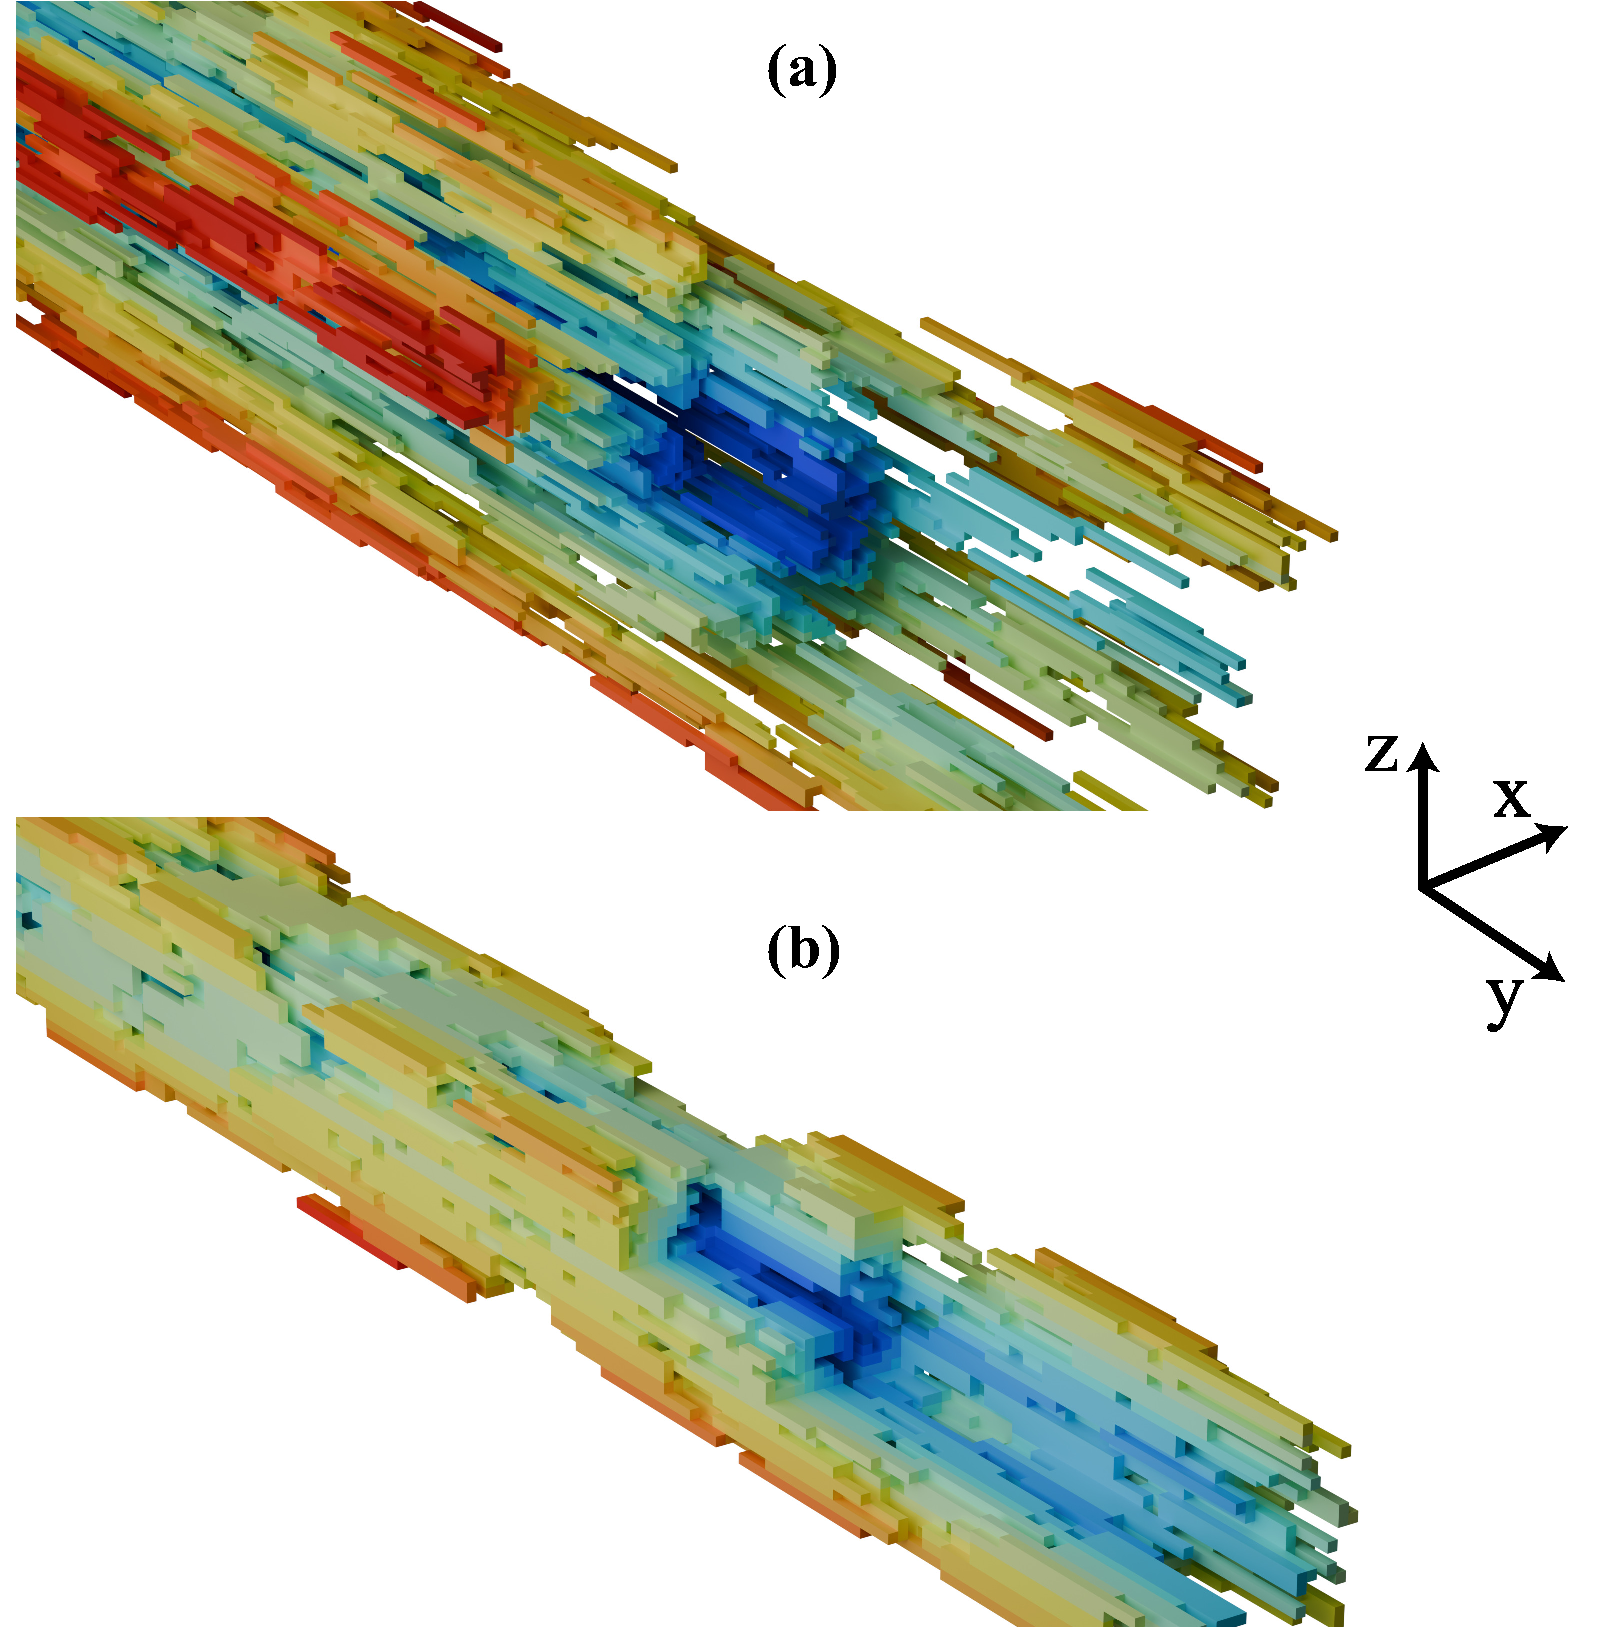
\includegraphics[width=0.7\textwidth]{figure_1.pdf}
	\caption{Representation of portions of fibrils generated with the DLA algorithm containing 30,000 molecules. Panels $(a)$ and $(b)$ show typical fibrils obtained with $T_s = 2$ (short-term diffusion) and $T_s = 8192$ (long-term diffusion), respectively. Colors indicate the relative time of attachment, from early (blue) to late (red).}
	\label{fig_1}
\end{figure}

The generated fibrils exhibit complex, heterogeneous packing with internal voids whose prevalence depends strongly on $T_s$ (Fig.~\ref{fig_1}). For $T_s = 2$, the fibril displays an open architecture with visible gaps between molecular clusters. In contrast, for $T_s = 8192$, the structure becomes more compact and homogeneous, with substantially reduced void space.

Although fibril growth proceeds primarily along the longitudinal axis ($y$-direction), the influence of the surface diffusion parameter $T_s$ is most pronounced in the radial organization of the structure ($x$-$z$ plane), as illustrated in Fig.~\ref{fig_2}. At low $T_s$ (Fig.~\ref{fig_2}a), the projected cross-sections are open and branched. As $T_s$ increases, however, the packing becomes progressively more compact and regular, reaching a highly uniform configuration at $T_s = 8192$ (Fig.~\ref{fig_2}d). Since a higher local packing density implies a greater number of intermolecular contacts, this morphological transition suggests that fibrils formed at larger $T_s$ exhibit enhanced connectivity and mechanical stability \cite{Mohammadkhah2023}.

\begin{figure}[!htb]
	\centering
	\includegraphics[width=1.\textwidth]{figure_2.pdf}
	\caption{Representative examples of projected central segments ($x$-$z$ plane) for different values of $T_s$: (a) $T_s = 2$, (b) $T_s = 64$, (c) $T_s = 512$, and (d) $T_s = 8192$. The progression illustrates a clear transition from sparse, irregular morphology at low $T_s$ to dense, radially symmetric packing at high $T_s$. The color gradient (blue to red) represents the temporal sequence of molecular incorporation, from early-attached to recently added molecules.}
	\label{fig_2}
\end{figure}

To quantify how $T_s$ modulates fibril structure, we estimated the fractal dimension of the central segment, defined as the region extending from $y=-100$ to $y=100$. For each $T_s$, we generated 50 fibrils and isolated this central region from each. Within each central segment, we extracted 11 cross-sections at intervals of $18~\text{l.u.}$ between $y=-90$ and $y=90$, yielding a total of 550 cross-sections per $T_s$ value. For each cross-section, we computed the center of mass and the maximum radius enclosing all particles; $R_{\text{max}}$ was subsequently defined as the largest of these 550 radii. The mass $m(R)$ was measured as the number of particles within a circular region of radius $R$ centered at the cross-section's center of mass. For each value of $R$ spanning from $R_{\text{min}} = 5~\text{l.u.}$ to $R_{\text{max}}$, we computed the mean mass $\langle m(R) \rangle$ by averaging over all 550 cross-sections \cite{Vicsek1991}. The fractal dimension $D_f$ was then extracted from the mass--radius scaling relation \cite{Giordano2012}:

\begin{equation}
	\langle m(R) \rangle \sim R^{D_{f}},
	\label{eq1}
\end{equation}
by performing a linear fit on a log-log plot of $\langle m(R) \rangle$ versus $R$.

As shown in Fig.~\ref{fig_3}, the fractal dimension $D_f$ depends strongly on $T_s$, providing a quantitative measure of the morphological transition observed in Fig.~\ref{fig_2}. For $T_s = 2$, we find $D_f = 1.708 \pm 0.005$, close to the characteristic value of two-dimensional diffusion-limited aggregation ($D_f \approx 1.71$) \cite{Witten1983}. As $T_s$ increases, $D_f$ rises and saturates at $D_f = 1.963 \pm 0.001$ for $T_s = 8192$, approaching the Euclidean limit $D_f = 2.0$ expected for a compact two-dimensional disk. Thus, increasing post-attachment mobility drives a crossover from diffusion-limited, fractal packing to nearly space-filling cross-sections.

\begin{figure}[h!]
	\centering
	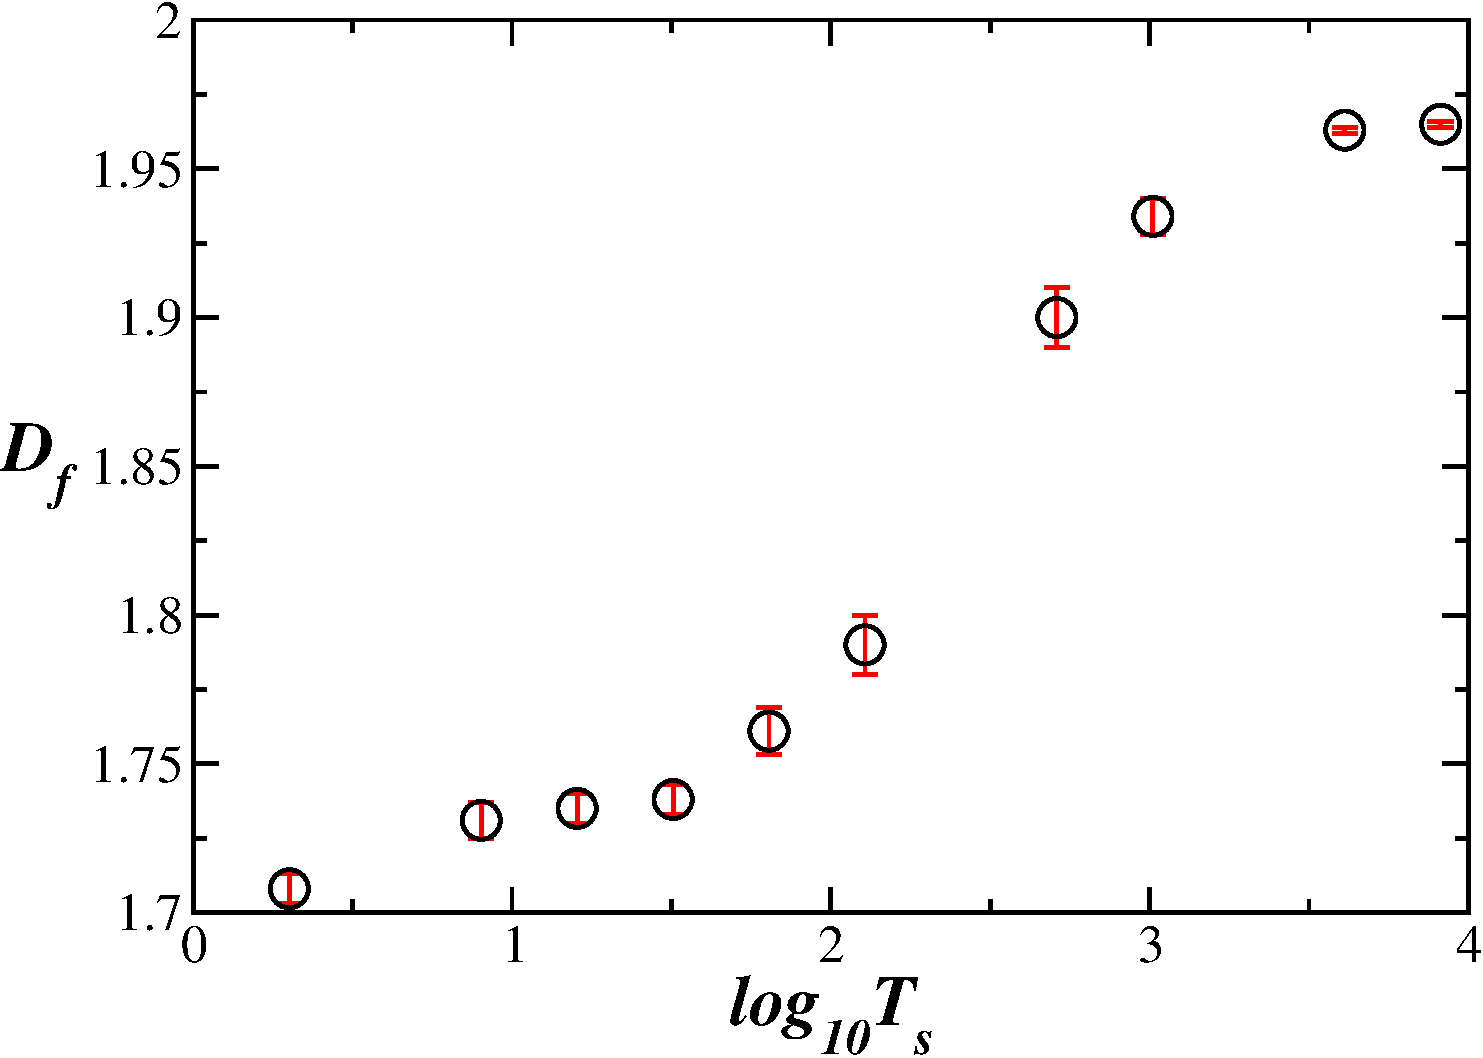
\includegraphics[width=0.7\textwidth]{figure_3.pdf}
	\caption{Average fractal dimension $D_f$ as a function of the diffusion parameter $T_s$ on a log-linear plot. Error bars are shown in red. The fractal dimension increases from $D_f = 1.708 \pm 0.005$ at $T_s = 2$ to $D_f = 1.963 \pm 0.001$ for $T_s = 8192$.}
	\label{fig_3}
\end{figure}		


\subsection{Mechanical Model for Fibril Rupture}

To connect the $T_s$-dependent fibril architecture to mechanical failure, we modeled rupture using a progressive, probabilistic fracture framework commonly employed for disordered networks \cite{z2019,Gilabert1987,Noguchi2024}. Because collagen molecules are represented as rigid rods that do not undergo continuous deformation prior to failure, we do not attempt to resolve deterministic crack propagation. Instead, intermolecular bonds fail stochastically under an applied axial force, and whole molecules detach from the load-bearing network with a stress-dependent probability. The procedure consists of:
$(i)$ isolating a trunk (force-carrying core) with dimensions $S_x = 17$, $S_y = 201$, and $S_z = 17$ l.u. \cite{Parkinson1997}. Truncation inevitably creates disconnected dangling ends that do not contribute to force transmission \cite{Herrmann1984}; we therefore
$(ii)$ identify the backbone (active skeleton) within the trunk prior to applying tensile loading \cite{Moreira2012}.

Backbone extraction proceeds in two passes. In the first pass, molecules at $y = 1$ are marked as active, and we scan upward to $y = S_y$, progressively marking molecules in contact with active ones; unmarked molecules are then removed. In the second pass, molecules at $y = S_y$ are marked as active, and we scan downward to $y = 1$ using the same connectivity rule; only molecules marked active after this pass are retained, defining the final backbone \cite{Parkinson1997} (Fig.~\ref{fig_4}).

\begin{figure}[h!]
	\centering
	
\includegraphics[width=\textwidth]{figure_4.pdf}
	\caption{(a) Two-dimensional visualization of an isolated fibril trunk used to extract the backbone. The circle highlights the region where the identification procedure starts ($y = 1$). (b) Example of the backbone identification procedure from left to right: molecules marked as active are highlighted in black as connectivity is propagated along the trunk, yielding the final backbone.}
	\label{fig_4}
\end{figure}

With the backbone identified, we simulate the effects of axial tension along the main axis ($y$) by progressively increasing a dimensionless force parameter $F$, where $F$ probabilistically governs molecular removal. At each cross-section $i$, we define the effective load-bearing area as the number of backbone segments intersecting that plane, $N(i)$. Each discrete segment is assigned unit area on the lattice \cite{Parkinson1995}; assuming uniform load sharing, the local tensile stress at cross-section $i$ is:

\begin{equation}
	\sigma(i) = \dfrac{F}{N(i)}.
	\label{eq2}
\end{equation}

We assume that failure occurs through rupture of intermolecular bonds, such that molecules detach intact rather than breaking internally \cite{Parkinson1997}. For a molecule spanning $n$ cross-sections, the mean stress is computed as the average of the local cross-sectional stresses:

\begin{equation}
	\sigma_{M} = \dfrac{1}{n}\sum_{i=1}^{n} \sigma(i).
	\label{eq3}
\end{equation}

A molecule's fracture resistance is taken to scale with the number of intermolecular contacts it forms within the backbone \cite{Vater1979}. For each molecule, we count first-neighbor contacts for every segment in each intersected cross-section and sum these contributions to obtain the total coordination number $K$. The corresponding failure threshold is $K\sigma_c$, where $\sigma_c$ is the critical stress for bond rupture; we set $\sigma_c = 1$, assuming identical molecules. To simplify the model, both the applied force parameter $F$ and the critical stress $\sigma_c$ are treated as dimensionless quantities in arbitrary units. Here, $\sigma_c = 1$ represents the normalized threshold for intermolecular bond rupture, allowing focus on relative mechanical behavior rather than absolute physical values.

The probability of removing a molecule is then:

\begin{equation}
	P_{R} = \left( \dfrac{\sigma_{M}}{K\sigma_c} \right)^{m},
	\label{eq4}
\end{equation}
where $m$ is the Weibull modulus (dimensionless shape parameter) that controls the amount of statistical scatter in this stochastic removal rule~\cite{Parkinson1997,Jones2012}. Larger $m$ yields a narrower distribution of effective rupture strengths (less variability), whereas smaller $m$ produces broader scatter. Here, we set $m = 2$ following the work of Parkinson et al.~\cite{Parkinson1997}. Fig.~\ref{fig_5} schematically illustrates the calculation of $\sigma(i)$, $\sigma_{M}$, and $K$ for a representative molecule.

\begin{figure}[ht!]
	\centering
	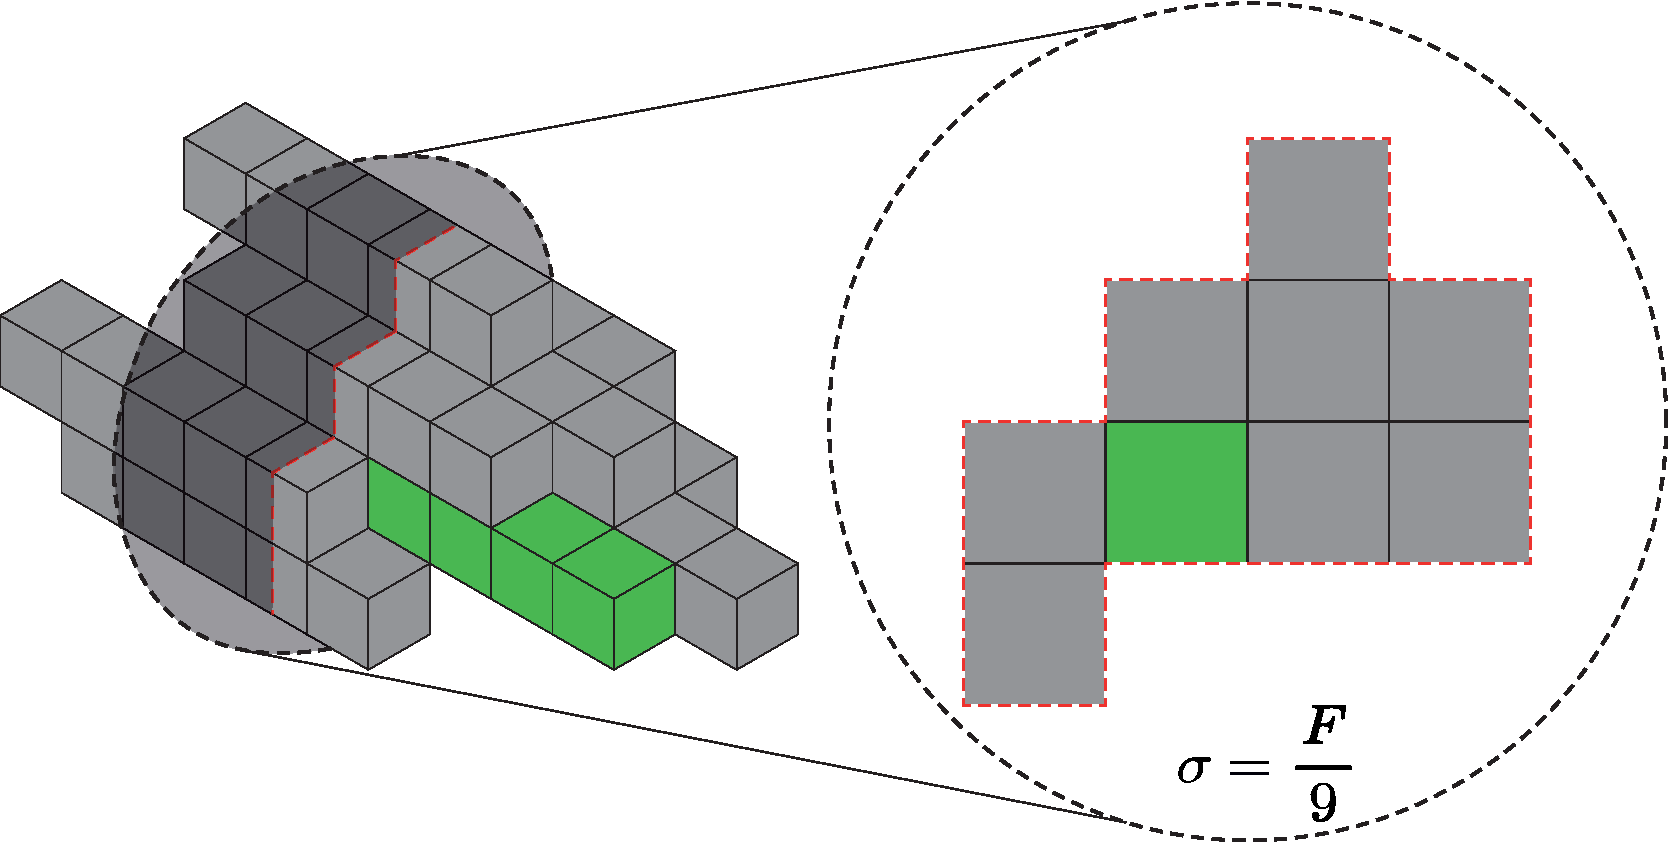
\includegraphics[width=0.9\textwidth]{figure_5.pdf}
	\caption{Schematic illustration of the computation of the removal probability $P_{R}$ for a representative molecule (blue). Left: a portion of the backbone where each rectangle represents a molecule (drawn with five segments for clarity). The blue molecule intersects multiple cross-sections; for each intersected cross-section $i$, the local stress is $\sigma(i)=F/N(i)$ (right; example with $N(i)=9$, giving $\sigma(i)=F/9$).}
	\label{fig_5}
\end{figure}

For a given force level $F$, we evaluate $P_{R}$ for every molecule in the backbone and compare it with an independent random number $u\in[0,1]$. If $u < P_{R}$, the molecule is removed. After each sweep, stresses and probabilities are recalculated for the remaining backbone, and the sweep is repeated until no additional removals occur. The applied force is then increased by $\Delta F = 0.5$, and the procedure is repeated. Rupture is defined as the appearance of a completely void cross-section, signaling failure of the backbone. The steps of this removal process are schematized in Fig.~\ref{fig_6}.

\begin{figure}[ht!]
	\centering
	\includegraphics[width=0.9\textwidth]{figure_6.pdf}
	\caption{Schematic view of the load-bearing backbone and the stages of the rupture process. (a) Two-dimensional view of the backbone subjected to an axial force $F$ along the $y$-axis. Each molecule (gray) is assigned a removal probability $P_{R}$ (Eq.~\ref{eq4}); a molecule is removed when a random number $u\in[0,1]$ satisfies $u<P_{R}$. (b) Progressive damage after some molecules have been removed, represented by red dashed lines. (c) Rupture occurs when a cross-section becomes completely empty (solid lines), eliminating the continuous load path.}
	\label{fig_6}
\end{figure}

Since our rupture model is probabilistic, for each value of $T_s$ we analyzed an ensemble of $10$ distinct fibrils, each containing $3\times 10^4$ molecules, and performed $10^3$ independent rupture simulations per fibril. During each simulation, the force was increased incrementally, and at each level we recorded the molecules removed from the backbone.

To quantify the mechanical resistance of the simulated fibrils, we analyzed the evolution of the average fraction of removed molecules, denoted by $\varphi$, as a function of the applied force $F$ \cite{Parkinson1997}. As shown in Fig.~\ref{fig_7}(a), $\varphi$ increases monotonically with $F$, reflecting progressive intermolecular bond rupture and loss of load-bearing connectivity.

The force threshold for rupture increases with $T_s$, consistent with enhanced connectivity in more compact fibrils. Despite different rupture thresholds, all curves exhibit a common functional form:

\begin{equation}
	f(F) = 10^{-3}\left[\exp(\beta F) -1 + F^{\alpha}\right],
	\label{eq5}
\end{equation}
where the coefficients $\alpha$ and $\beta$ are determined from fits to the data by using Eq.~(\ref{eq5}). At low forces, the response is dominated by the power-law term, corresponding to gradual damage accumulation. Close to rupture, the exponential term dominates, producing a rapid increase in $\varphi$ \cite{Buehler2009}. Fig.~\ref{fig_7}(b) and Fig.~\ref{fig_7}(c) show that both $\alpha$ and $\beta$ decrease with $T_s$ and stabilize for $T_s \geq 512$. The parameter $\alpha$ sets the rate of gradual (power-law) damage accumulation \cite{Veres2013}, whereas $\beta$ controls the onset of rapid, avalanche-driven failure \cite{Zapperi1997a,Zapperi1999}.

\begin{figure}[ht!]
	\centering
	
\includegraphics[width=\textwidth]{figure_7.pdf}
	\caption{(a) Average fraction of removed molecules $\varphi$ versus applied force $F$ for $T_s = 8, 32, 128$, and $8192$. Solid lines are fits to $f(F) = 10^{-3}[\exp(\beta F) -1 + F^{\alpha}]$. (b) and (c) Fitted parameters $\beta$ and $\alpha$ as a function of $T_s$; both decrease and saturate for $T_s \geq 512$.}
	\label{fig_7}
\end{figure}

During rupture, molecules detach either individually or in spatially connected clusters removed during the same force increment. We define a cluster as any group of two or more adjacent molecules removed at the same force step. Such cluster detachments correspond to avalanches, a hallmark of crackling dynamics in driven disordered systems \cite{Jaeger1992,Godano1993,Beggs2003,Baraba1996,Alencar2001,Suki1994}. To quantify the importance of collective events, we introduce $\Psi$, defined as the fraction of removed molecules that belong to clusters relative to the total number removed at a given force level. To compare across different rupture forces, we express the force as a normalized variable $F_n = F/F_{\mathrm{rup}}$, where $F_{\mathrm{rup}}$ is the rupture force of each realization. As shown in Fig.~\ref{fig_8}, low-$T_s$ fibrils exhibit large $\Psi$ even at small $F_n$, indicating early collective failure, whereas high-$T_s$ fibrils primarily fail through isolated removals until close to rupture, when $\Psi$ rises sharply.


\begin{figure}[ht!]
	\centering
	
\includegraphics[width=0.7\textwidth]{figure_8.pdf}
	\caption{The average fraction of molecules removed in a cluster, $\Psi$, as a function of normalized force $F_n = F/F_{\mathrm{rup}}$ for $T_s = 8, 32, 128$ and $8192$. For low $T_s$, cluster breakages contribute significantly even at low forces, indicating early onset of collective failure. In contrast, for high $T_s$, the fibril initially resists through isolated bond breaking, with cluster breakages (and catastrophic failure) occurring only near rupture.}
	\label{fig_8}
\end{figure}

To understand this collective behavior, we analyze it from the viewpoint of avalanche statistics~\cite{Bak1987}. Here, we define the avalanche size, $s$, as the cluster size, i.e., the number of molecules in a removed cluster at a fixed force level. We then compute $P(s)$, the probability distribution of avalanche sizes, for each value of $T_s$. The inset of Fig.~\ref{fig_9}(a) shows representative distributions for $T_s=2$ and $T_s=8192$. To characterize these distributions, we apply the scaling law~\cite{Zapperi1997b}:

\begin{equation}
	P(s) \sim s^{-\gamma},
	\label{eq6}
\end{equation}
where $\gamma$ is the characteristic exponent of the power law.

The main panel in Fig.~\ref{fig_9}(a) shows the scaling regime where this power-law behavior provides a good fit over two orders of magnitude. Our analysis yields $\gamma=2.31\pm 0.05$ for $T_s = 2$ and $\gamma=2.80\pm0.04$ for $T_s=8192$. Between these limits, $\gamma$ varies systematically with $T_s$ (Fig.~\ref{fig_9}b): it increases approximately linearly with $\log(T_s)$ for $T_s < 512$ and reaches a plateau for $T_s \geq 512$.

In many stochastic fracture and fiber-bundle models, the avalanche exponent $\gamma$ is sensitive to the reach of stress redistribution following a local failure event, with a crossover from local to global load sharing \cite{Daniels1945,Hemmer1992,Hansen1994,Kloster1997,Zapperi1999,Kun2000,Pradhan2010}. In our fibrils, increasing $T_s$ drives a structural transition toward compact packing (larger $D_f$, Fig.~\ref{fig_3}), implying a denser, more highly connected backbone and hence a larger effective stiffness $\kappa_{\mathrm{eff}}$. Since Eq.~(\ref{eq1}) implies that in a $d=2$ cross-section $\rho(R)\sim \langle m(R)\rangle/R^2 \sim R^{D_f-2}$, the approach $D_f\to2$ corresponds to an increasingly space-filling morphology with weak scale dependence of $\rho$. A larger $\kappa_{\mathrm{eff}}$ enables broader stress redistribution, de-correlates rupture events, and suppresses system-spanning avalanches, making small failure events more frequent relative to large ones and thereby increasing $\gamma$ \cite{Bak1987,Hidalgo2002,Pradhan2005,Biswas2013,Danku2018,Zhao2025}. Consistent with this interpretation, the saturation of $\gamma$ for $T_s \ge 512$ coincides with $D_f \gtrsim 1.90$ and with the stabilization of the fit parameters $\alpha$ and $\beta$ (Fig.~\ref{fig_7}), suggesting diminishing sensitivity of the failure statistics to further surface relaxation. Futhermore, the systematic increase in $\gamma$ with $T_s$ signals a fundamental shift in the system's criticality: the transition from fractal to compact architecture progressively screens long-range elastic interactions, driving the failure dynamics toward a regime dominated by small-scale stochastic events and thus pointing to a change in universality class.

\begin{figure}[ht!]
	\centering
	
\includegraphics[width=\textwidth]{figure_9.pdf}
	\caption{(a) Log-log plot of the rupture avalanche size distribution, $P(s)$, as a function of avalanche size $s$ for $T_s = 2, 32, 128$ and $8192$. A power-law regime $P(s) \sim s^{-\gamma}$ is observed, with slopes $\gamma$ ranging from $2.31\pm0.04$ ($T_{s}=2$) to $2.80\pm0.05$ ($T_{s}=8192$) obtained from the linear fit (solid lines) following the scaling behavior. The inset shows the full distributions, including the tails, for $T_s = 2$ and $T_s = 8192$. The avalanche size distributions are vertically shifted for better visualization. In (b) the exponent $\gamma$ as a function of $T_s$ on a log-linear scale, showing two regimes: growth for $T_s < 512$ and a plateau for $T_s \geq 512$.}
	\label{fig_9}
\end{figure}

A direct consequence of avalanche-like rupture should be sudden stress drops in stress--strain curves, since avalanches propagate faster than the imposed loading rate \cite{Noguchi2024}. Although our model does not resolve continuous strain and thus cannot generate stress--strain curves, experimental evidence strongly supports this prediction. Gutsmann et al. \cite{Gutsmann2004} used force spectroscopy on single microfibrils and directly observed force drops caused by intermolecular cross-link rupture. Svensson et al. \cite{Svensson2013} reported clear stress drops in tensile tests of individual collagen fibrils, while Deng et al. \cite{Deng2024} observed similar drops in stress--strain curves.

Our coarse-grained framework represents collagen molecules as rigid rods with restricted aggregation and no rotational diffusion. Intermolecular interactions are simplified via $T_s$, which lacks a direct mapping to biochemical conditions like pH \cite{Jiang2004}. Fracture is implemented probabilistically, omitting detailed force transmission and internal bond-breaking mechanics \cite{RuizFranco2022,Provenzano2006}. Consequently, the model does not produce stress--strain curves or elastic moduli \cite{Innocenti2022-lp}. Nevertheless, it reveals that rupture follows scale-free avalanche dynamics and that structural compactness correlates with mechanical resilience. Thus, the fractal dimension serves as a quantitative bridge between assembly conditions and failure statistics in these biomaterials.

\section{Conclusion}

In this work, we combined a three-dimensional diffusion-limited aggregation model of collagen fibrillogenesis with a progressive probabilistic rupture model to connect assembly kinetics, fibril architecture, and failure statistics. Increasing the post-attachment surface diffusion parameter $T_s$ drives a clear morphological crossover from porous, fractal packing to nearly compact cross-sections: the measured fractal dimension rises from $D_f=1.708\pm0.005$ at $T_s=2$ to $D_f=1.963\pm0.001$ at $T_s=8192$. Mechanically, more compact fibrils exhibit higher rupture thresholds and a delayed onset of collective failure, while the avalanche size distribution remains scale-free, $P(s)\sim s^{-\gamma}$. Importantly, the avalanche exponent increases systematically with $T_s$, from $\gamma=2.31\pm0.05$ ($T_s=2$) to $\gamma=2.80\pm0.04$ ($T_s=8192$), with a plateau for $T_s\ge 512$ that coincides with $D_f\gtrsim 1.90$ and with saturation of the damage-fit parameters $\alpha$ and $\beta$.

From a physical perspective, the joint increase of $D_f$ and $\gamma$ indicates that densification of the load-bearing backbone promotes more homogeneous stress redistribution, shifting the rupture dynamics away from correlated, system-spanning avalanches and toward a regime dominated by smaller events, consistent with a crossover in the effective universality class. 

In the framework of fiber-bundle models, the exponent $\gamma=5/2$ is the exact mean-field result for equal load sharing (ELS) \cite{Hemmer1992,Hansen1994,Kloster1997}, whereas local load sharing (LLS) yields lower, non-universal exponents that depend on dimensionality and disorder \cite{Hidalgo2002,Pradhan2005,Biswas2013,Danku2018}. Our measured exponents evolve from $\gamma\approx 2.3$ at low $T_s$---below the ELS value and thus closer to the LLS regime---to $\gamma\approx 2.8$ at high $T_s$, exceeding $5/2$ and approaching the behavior expected when stress redistribution becomes effectively global \cite{Pradhan2010}. This progression suggests that increasing structural compactness extends the range of load redistribution within the fibril, driving a genuine transition from local to global load-sharing universality. 

From an application standpoint, this provides a simple route to tune mechanical resilience in collagen-based fibers and biomaterials by controlling assembly conditions that regulate compactness. While our framework is intentionally coarse-grained (rigid lattice rods, phenomenological $T_s$, and probabilistic failure with simplified load transfer), it offers a minimal, quantitative link between fibril geometry (via $D_f$) and failure statistics (via $\gamma$), helping rationalize how microstructural remodeling impacts macroscopic robustness. Future work should incorporate more realistic mechanics and time dependence---including elastic or viscoelastic deformation and evolving stiffness (e.g., due to cross-link dynamics or degradation)---to predict stress--strain behavior and track how the fiber modulus changes over time under load.

\section{Author Contributions}
All authors contributed equally to this work.

\section{Acknowledgments}
We thank the Brazilian agencies CNPq, CAPES, and FUNCAP for financial support.


% If in two-column mode, this environment will change to single-column
% format so that long equations can be displayed. Use
% sparingly.
%\begin{widetext}
% put long equation here
%\end{widetext}

% figures should be put into the text as floats.
% Use the graphics or graphicx packages (distributed with LaTeX2e)
% and the \includegraphics macro defined in those packages.
% See the LaTeX Graphics Companion by Michel Goosens, Sebastian Rahtz,
% and Frank Mittelbach for instance.
%
% Here is an example of the general form of a figure:
% Fill in the caption in the braces of the \caption{} command. Put the label
% that you will use with \ref{} command in the braces of the \label{} command.
% Use the figure* environment if the figure should span across the
% entire page. There is no need to do explicit centering.

% \begin{figure}
% \includegraphics{}%
% \caption{\label{}}
% \end{figure}

% Surround figure environment with turnpage environment for landscape
% figure
% \begin{turnpage}
% \begin{figure}
% \includegraphics{}%
% \caption{\label{}}
% \end{figure}
% \end{turnpage}

% tables should appear as floats within the text
%
% Here is an example of the general form of a table:
% Fill in the caption in the braces of the \caption{} command. Put the label
% that you will use with \ref{} command in the braces of the \label{} command.
% Insert the column specifiers (l, r, c, d, etc.) in the empty braces of the
% \begin{tabular}{} command.
% The ruledtabular enviroment adds doubled rules to table and sets a
% reasonable default table settings.
% Use the table* environment to get a full-width table in two-column
% Add \usepackage{longtable} and the longtable (or longtable*}
% environment for nicely formatted long tables. Or use the the [H]
% placement option to break a long table (with less control than 
% in longtable).
% \begin{table}%[H] add [H] placement to break table across pages
% \caption{\label{}}
% \begin{ruledtabular}
% \begin{tabular}{}
% Lines of table here ending with \\
% \end{tabular}
% \end{ruledtabular}
% \end{table}

% Surround table environment with turnpage environment for landscape
% table
% \begin{turnpage}
% \begin{table}
% \caption{\label{}}
% \begin{ruledtabular}
% \begin{tabular}{}
% \end{tabular}
% \end{ruledtabular}
% \end{table}
% \end{turnpage}

% Specify following sections are appendices. Use \appendix* if there
% only one appendix.
%\appendix
%\section{}

% If you have acknowledgments, this puts in the proper section head.
%\begin{acknowledgments}
% put your acknowledgments here.
%\end{acknowledgments}

% Create the reference section using BibTeX:
\bibliography{apssamp}

\end{document}
%
% ****** End of file apstemplate.tex ******
